\chapter{Pilot-Wave Hydrodynamics}
\label{Ch1}

In this chapter I will present a brief survey of the literature describing the hydrodynamic quantum analog, and discuss in more detail the particular tunneling experiments relevant to my investigation. Because the system was discovered in 2005, most of the literature examining this topic was written within the last ten years.


\section{Oil Droplet System}
	    \label{parameters}
	       Consider a fluid of density $\rho$, viscosity $\nu$, and surface tension $\sigma$ in a bath of depth $H$. The bath is sinusoidally driven vertically at an amplitude $A_0$ at a frequency $f=\omega/{2\pi}$. By defining $\mathnormal{\gamma}=A_0\omega^2$, the effective gravity in the frame of reference of the bath is $g+\gamma~\mathrm{sin}(\omega t)$. The surface of oil in the shaking tray remains quiescent for lower values of $\gamma$. However, if  $\gamma$ is increased (by increasing $A_0$ or $f$), the surface becomes unstable leading to the appearance of standing surface waves called Faraday waves. We define the threshold at which these waves appear as the \textbf{Faraday threshold}, $\gamma_\mathrm{F}$. The value of $\gamma_\mathrm{F}$ changes depending on the size and shape of the tray, the amount of fluid in the tray, and the properties of the fluid. 
	       
	   \begin{figure}[h]
	       \centering
	    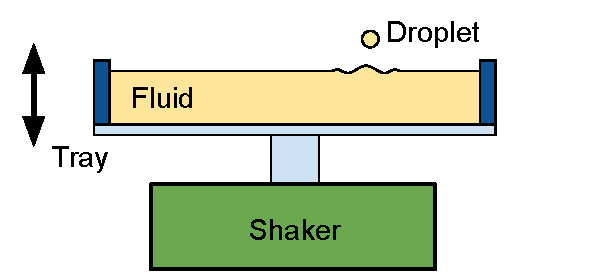
\includegraphics[scale=.80]{basicsetup.pdf}
	     \caption{A droplet bounces on a vertically vibrating fluid bath. The tray vibrates with an amplitude $A_0$ at frequency $f$.}
	 \label{basic}
	\end{figure}
	       
	    If we take a toothpick and break the surface of the vibrating oil bath, we form a droplet of oil of diameter $D$ as shown in \refFig{basic} which bounces on the surface for hours. The droplet bounces on a pocket of air, which is trapped beneath the droplet and the bath~\rf{Walker}. As the oil droplet bounces, it creates radially traveling waves that propagate outwards in an otherwise flat surface. The droplet will continue bouncing for a specific range of values of $\gamma$. For a small $\gamma$, the forcing is not enough to sustain the droplet, and it quickly coalesces. Increasing $\gamma$ above the threshold for coalescence leads to a variety of different bouncing regimes until at $\gamma = \gamma_\mathrm{F}$ where Faraday waves emerge. Below $\gamma_\mathrm{F}$, value of $\gamma$ also affects they range of the radial waves; for low $\gamma$ these waves quickly dissipate, and for values of $\gamma$ that approach $\gamma_\mathrm{F}$ they are sustained longer. We are interested in studying the region below the appearance of Faraday waves but above the region of coalescence. The range of the various parameters which allow for the existence of the bouncing droplet are outlined in \refTab{approxlimits} \cite{pilot-wave}. 
	      
	       \begin{table}[htdp] 
\caption[Basic Table 1]{Approximate limits for bouncing drop behavior. The value $g = 9.81~\mathrm{m/s}^{2}$ is the standard acceleration due to gravity.} 
\begin{center} 
\begin{tabular}{c c c} 
\toprule 
  Parameter &  Lower Limit & Upper Limit \\
  \midrule
Viscocity $\nu$ (cSt) & 10 & 100 \\ 
Bath Depth $H$ (mm) & 4 & 10 \\
Frequency $f$ (Hz) & 20 & 150 \\
Amplitude $A_0$ (mm) & 0.1 & 1 \\
Drop Diameter $D$ (mm) & 0.6 & 1.0 \\
Forcing Acceleration $\gamma$ ($\mathrm{ms}^{-2}$) & 0.5$g$ & $\gamma_\mathrm{F} \approx 4.2g$ \\
\bottomrule 
\end{tabular}
\end{center}
\label{approxlimits} 
\end{table}	

\subsection{Faraday Waves}
Driving a fluid-filled tray with forcing acceleration $\gamma = \gamma_\mathrm{F}$ we see the appearance of standing surface waves known as Faraday waves. These waves oscillated with a  frequency $f_\mathrm{F} = f/2$ and an angular frequency $\omega_\mathrm{F} = 2\pi f_\mathrm{F}=\pi f$. For a fluid bath of density $\rho$, surface tension $\sigma$, and height $H$, the standing wave and water dispersion relation can be used to find the wavelengths of standing waves at the Faraday threshold:
\begin{equation} \label{dispersion}
\omega_\mathrm{F}^2 = \left(gk_\mathrm{F}+\frac{\sigma k_\mathrm{F}^3}{\rho}\right)\mathrm{tanh}(k_\mathrm{F}H),
\end{equation} 
which relates the angular Faraday frequency $\omega_\mathrm{F}$ to the Faraday wavenumber $k_\mathrm{F}$, where $g$ is the gravitational constant \rf{Kumar1996}. From the wavenumber, we can calculate the wavelength $\lambda_\mathrm{F}$ of the Faraday waves by the relation $\lambda_\mathrm{F}$ = $2\pi/k_\mathrm{F}$. Though we are interested in investigating the region $\gamma < \gamma_\mathrm{F}$ for which there are no standing surface waves, \refeq{dispersion} provides an estimate to the wavelength and frequency of the localized waves surrounding the droplet for the bouncing behavior. 


\subsection{Vibration Number}

In an experiment of this nature, one usually pours a specific volume of oil in the tray, fixing the values of $\nu$, $\sigma$, and $H$. One is then left with the option to adjust $\gamma$ which produces a range of droplet motions, including a slew of different stationary bouncing modes and linear or chaotic ``walking" trajectories (which are discussed in \refSect{sect:walking}). To visualize the various bouncing behaviors, we use the vibration number $V_i$, which takes into account many of the parameters of the experiment \rf{Molacek2013}. The vibration number is the ratio of the forcing frequency and the drop's natural oscillation frequency:
\begin{equation} \label{vibrationnumber1}
V_i = \frac{\omega}{\omega_\mathrm{D}}
\end{equation}   
where $\omega_\mathrm{D}$ represents the oscillation frequency of a fluid droplet. Rather than remain a perfect sphere, the droplet stretches and contracts vertically as it bounces, and $\omega_\mathrm{D}$ describes the frequency of this motion. The oscillation frequency of a fluid droplet is defined as:
\begin{equation} \label{oscillationfrequency}
\omega_\mathrm{D} = 2\sqrt{\frac{2\sigma}{\rho D^3}},
\end{equation}   
with surface tension $\sigma$, density $\rho$, and diameter of the droplet $D$ \rf{lord}. Combining \refeqs{vibrationnumber1}{oscillationfrequency} we arrive at:
\begin{equation} \label{vibrationnumber2}
V_i = \frac{\omega}{2}\sqrt{\frac{\rho D^3}{2\sigma}},
\end{equation}   	       	       
a dimensionless parameter that captures the fluid's surface tension $\sigma$ and density $\rho$, the tray's vibration $\omega$, and the droplet's diameter $D$. Depending on the vibration number $V_i$ and the driving frequency $\gamma/g$ the droplets switch between different bouncing states as shown in \refFig{regime}. If we hold the fluid and the driving frequency constant ($\sigma$, $\rho$, and $\omega$), then we can think of increasing $V_i$ as increasing droplet diameter $D$. 
	    
	    \begin{figure}[h]
	% the options are h = here, t = top, b = bottom, p = page of figures.
	% you can add an exclamation mark to make it try harder, and multiple
	% options if you have an order of preference, e.g.
	% \begin{figure}[h!tbp]
	       \centering
	    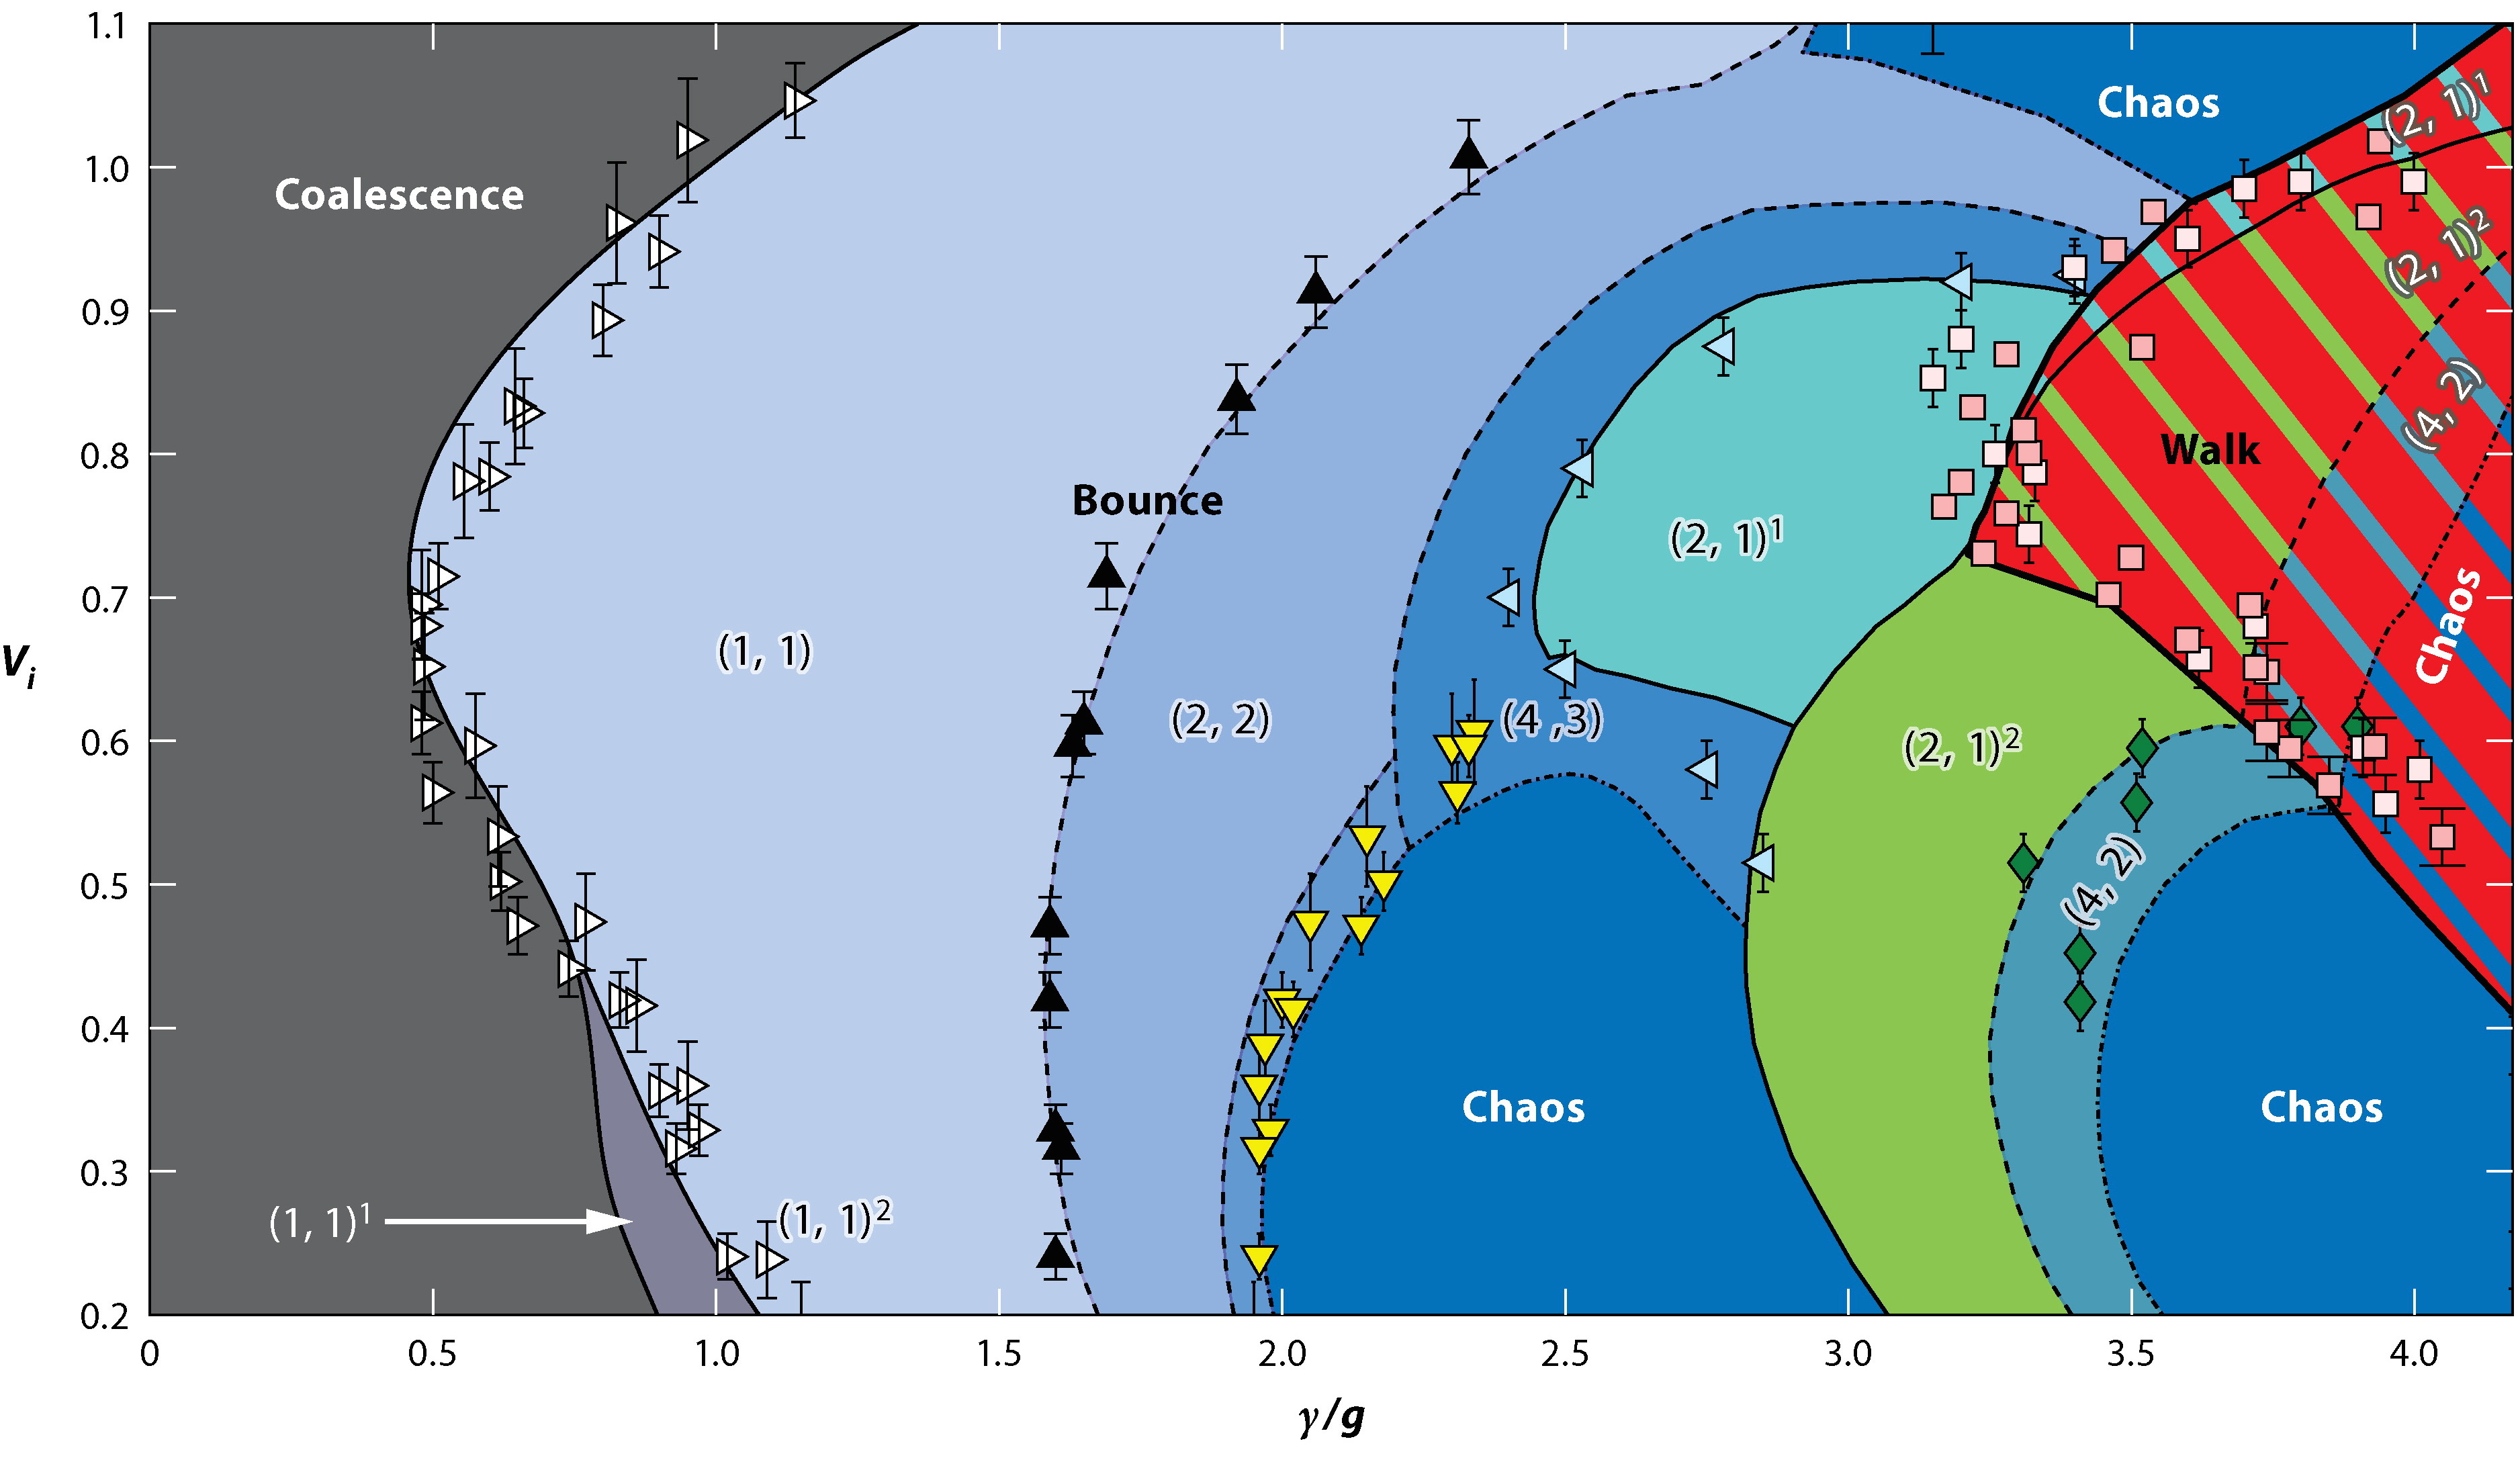
\includegraphics[scale=.1155]{vibrationnumber}
	     \caption{The different bouncing regimes for the oil drops of 20 cSt silicone oil at $f$ = $\omega / 2\pi$ = 80 Hz, characterized by the non-dimensionalized forcing frequency $\gamma/g$ and the vibration number $V_i$. The solid colors represent the  modes predicted by a theoretical model~\rf{Molacek2013}, and the various points represent experimentally measured limits. The parameters $(m,n)^{i}$ describe a droplet that bounces $n$ times in $m$ forcing periods, where $i$ distinguishes modes with different mechanical energy. The Faraday threshold is $\gamma_\mathrm{F} = 4.2$. Adapted from J. W. M. Bush, J. Fluid Mech. \textbf{727}, 273 (2014).}
	 \label{regime}
	\end{figure}

The various modes seen in \refFig{regime} can be described by a pair of numbers~$m$ and $n$, where $n$ is the number times the droplet contacts the surface over a time span $m/f$. For example, in the (1,1) ``bounce" mode, the droplet hits the oil bath once per up-and-down motion of the tray. In the (2,2) mode, the drop makes two bounces of differing heights for two driving periods. The ``chaos" regimes indicate that the bouncing of the droplet is chaotic, and it does not seem to exhibit a periodic bouncing motion. The ``walk" regime describes a very particular kind of behavior in which the droplet moves forward as it bounces, seemingly walking across the surface. Like bouncing, walking also comes either the (2, 1), (4, 2), or the chaos mode. Finally, the ``coalescence" region demarcates the values for which the droplet coalesces with the bath.

The phase diagram shown in \refFig{regime} provides a valuable starting place for an experiment since it outlines the many possible states of the system, and where we can expect to find particular behaviors. We will now narrow our focus to only the walking regime, the bread and butter of this thesis.

	        \subsection{Walking}
	        \label{sect:walking}
A walking droplet is a very specific type of bouncing droplet that arises between $\gamma_\mathrm{W}~<~\gamma~<~\gamma_\mathrm{F}$. As the droplet bounces vertically on the vibrating fluid bath, the interaction with the wave it generated on it's previous bounce gives it a slight horizontal motion. Thus, for every bounce, the droplet follows a parabolic trajectory. But because these droplets are bouncing at 40 times per second (or more) and the parabolic motion is periodic, the vertical oscillations are difficult to see. The apparent behavior that emerges is that of the droplet moving in a straight line along the surface of the fluid bath.             

 \begin{figure}[h]
	       \centering
	    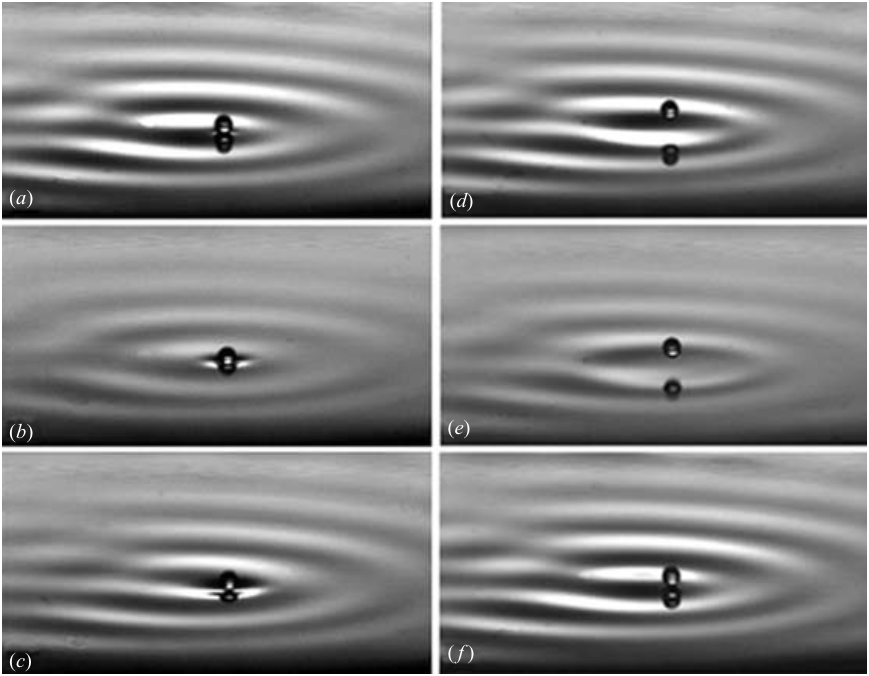
\includegraphics[scale=.495]{ProtiereWalkers}
	     \caption{%The series of pictures (a) - (c) show a droplet bouncing off of the slope of the localized wave, launching into the air, and then falling again on a new wave slope. This periodic process happens multiple times per second, giving the droplet the appearance of walking across the surface. Figure adapted from~\rf{Couder2005b}.
	    The series of pictures (a) - (f) show a walker over two forcing periods. The droplet bounces off of the slope of the localized wave, launching into the air, and then falls again on a new wave slope. This periodic process happens multiple times per second, giving the droplet the appearance of walking across the surface. Figure from S. Protiere, J. Fluid Mech. \textbf{554}, 93 (2006).
	     }
	 \label{Couderwalkers}
	\end{figure}
 
 
The horizontal component of the walking motion is due to the droplet landing slightly off center of the radial wave it produced in the previous bounce, shown in \refFig{Couderwalkers}. At such close proximity to the Faraday threshold, the waves surrounding the droplet are not just regular ripples, but rather are like localized Faraday waves temporarily sustained by the vibrations before decaying away. The kinetic energy from the falling droplet is enough to perturb the unstable surface such that the waves appear, and then the energy introduced by the vertical forcing of the tray keeps these waves from damping out completely, as they would in an un-forced system. The value of $\gamma$ determines how long these local Faraday waves are sustained. As these waves interfere with one another they create an overall wave field that guides the droplet. This overall wave field is referred to as the \textbf{guiding wave} or the \textbf{pilot wave}. A \textbf{walker} is defined as a self-propelling droplet \textit{and} its guiding wave, since they are mutually interdependent; the droplet creates the guiding wave, and the guiding wave moves the droplet. The unique combination of the two components results in novel interactions like bound or scattering states.


%For example, as a walker approaches the wall of the tray, the droplet will slow down as it approaches and then--without touching the wall--walk off in the other direction. What's actually happening is that the guiding wave reflects off of the wall, which creates a new pilot-wave that pushes the droplet away from the wall. The defining quality illustrated in this example is that the droplet is apparently influenced by another feature without touching it, the interaction is happening with the guiding wave.

 \subsubsection{Bound States}

\begin{figure}[h]
	       \centering
	    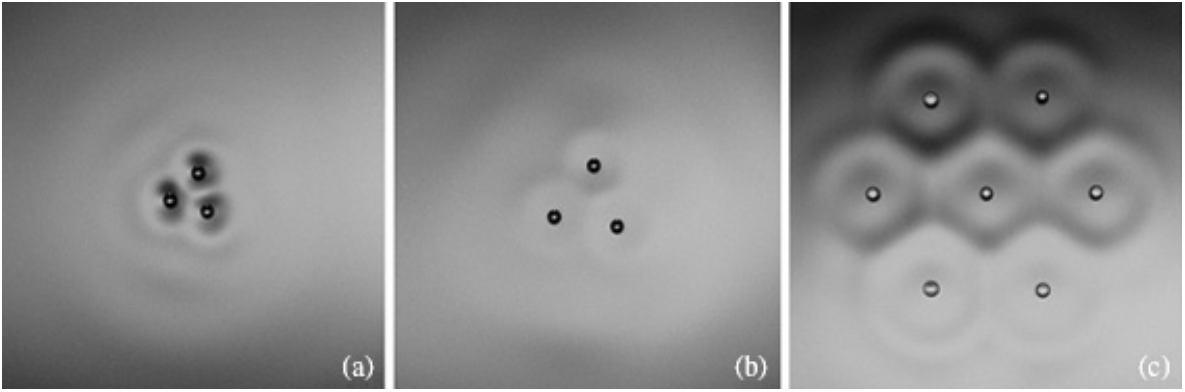
\includegraphics[scale=.366]{BoundedStates}
	     \caption{In (a), the trio of droplets organize themselves into a triangular lattice separated by distance $d_{0}^{bd}$. The forcing acceleration has been increased in (b), and the droplets are more spread out with a larger $d_{0}^{bd}$ value. Bound states can include a large number of bouncing droplets, as demonstrated by the 7 bouncing droplets shown in (c).   
	    Figure from S. Protiere, J. Phys.: Condens. Matter \textbf{17}, S3532 (2005). 
	     }
	 \label{bounded}
	\end{figure}
            A periodic damped wave allows for two bouncers to form a \textbf{bound state}: a configuration in which the droplets remain a fixed distance apart \rf{Protiere2005}.  Starting far away from one another, two droplets drift towards one another until a fixed distance $d_{0}^{bd}$. Increasing driving acceleration $\gamma$ will decrease their separation distance $d_{0}^{bd}$ (\refFig{bounded}). These bound bouncers can form triangular lattices, though their periodicity is highly sensitive to the mass of the droplet. If the masses of the droplets differ, these configurations drift slowly and rotate because the waves produced by the larger droplet are larger creating an imbalanced wave field \rf{Eddi2008}. Finally, the droplets can bounce in phase with one another (they both land at the same time and reach their peaks at the same time) or completely out of phase with one another (as one lands, the other reaches it's peak).
            
\begin{figure}[h]
	       \centering
	    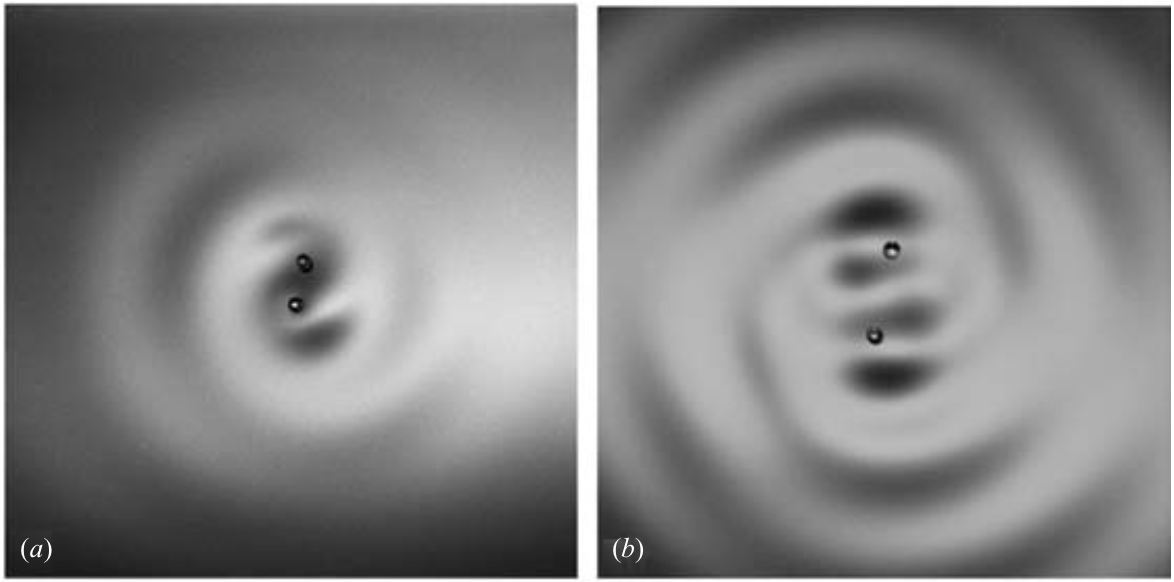
\includegraphics[scale=.33]{OrbitingProtiere2006}
	     \caption{ The figures show two droplets of equal size orbiting their center of mass. In (a) the droplets bounce out of phase with $n = 0.5$ and $d_{n}^{orb} =1.65~\mathrm{mm}$ whereas in (b) the droplets bounce in phase with  $n=1$ and  $d_{n}^{orb} = 3.7~\mathrm{mm}$.
	    Figure adapted from S. Protiere, J. Fluid Mech. \textbf{554}, 101 (2006). 
	     }
	 \label{orbiting}
	\end{figure}
 

            Walkers can also form bound states. Two walkers of the same size that are approaching one another can form an orbit around their center of mass as shown in \refFig{orbiting}. Between the two droplets is the fixed distance $d_{n}^{orb}$ given by          
\begin{equation} \label{orbital}
d_{n}^{orb} = (n - \epsilon_0)\lambda_F
\end{equation}         
where $\lambda_\mathrm{F}$ is the wavelength of the localized Faraday waves estimated by \refeq{dispersion}, $\epsilon_0$ is a fixed distance which is the same for all orbitals of these walkers (usually in the range $0.15 < \epsilon_0 < 0.25$ depending on droplet diameter), and $n = 1,2,3,...$ for drops that are in phase or $n = 1/2, 3/2, 5/2,...$ for drops out of phase. Orbiting periods are approximately proportional to $d_{n}^{orb}$, which ends up meaning that the velocity of the orbiting walkers is a little less than the velocity of a free walker \rf{Protiere2006}. 


            \subsubsection{Scattering States}
            Two identical walkers headed towards each other can form fixed orbits, or they can scatter. \textbf{Scattering} describes an interaction in which droplets are deflected through their wave fields, and never actually make contact with one another. Most of the interactions of a walker are scattering of some form. For example, if a single walker approaches the wall of the tray, it will never actually touch the wall. Instead, the guiding wave reflects off of the wall and modifies the wave field such the droplet will scatter in the opposite direction.           

%When two walkers interact with one another, their guiding waves interfere. Bouncing droplets will often organize themselves into stable configurations a specified distance apart. Increasing the forcing acceleration $\gamma$ will increase the separation between each droplet in the configuration. For walkers that 

%Walkers can travel anywhere from $5$ to $15~\mathrm{mm/s}$, depending on their size and on the driving acceleration $\gamma$ \rf{Protiere2005}.



 
            \subsection{Path Memory}
                        
            How close the system is to the Faraday threshold is captured by a parameter called path memory. This captures the importance of damping in the system \rf{Eddi2011}. Every time the droplet impacts the bath, it creates a radial traveling wave. Over the course of many bounces, a guiding wave field composed of a superposition of the many waves arises. In this way the wave field ``remembers" previous interactions, but is at the same time being periodically ``updated" with every new bounce of the droplet. Because droplet motion is influenced by the wave field, controlling the damping of the wave field will influence the path of the walker. 
            
For a bouncing droplet in which the guiding waves decay relatively quickly, the droplet can only be influenced by relatively recent waves. This kind of behavior is characterized as a low memory. Conversely, a high memory system is one in which waves do not decay quickly; they propagate outwards and reflect off of the surfaces of the tray before reflecting back and interfering with the other waves produced by the droplet. As one gets closer to the Faraday threshold, one achieves higher and higher memory because waves last longer. The quantum-like features described here arise in the high-memory limit. 

The non-dimensional memory parameter is formally defined as:
$$M_e = \frac{T_\mathrm{d}}{T_\mathrm{F}(1-\gamma/\gamma_\mathrm{F})},$$
where $T_\mathrm{d}$ is the decay time of waves in the absence of vibration and $T_\mathrm{F}$ is the period of the Faraday waves ($T_\mathrm{F} = 1/f_\mathrm{F}$) \rf{Harris2013}. It will suffice to discuss memory as a fraction of the Faraday threshold $\gamma/\gamma_{F}$, since the fraction and $M_e$ are monotonically related. As the value of $\gamma/\gamma_{F}$ increases we get closer to the Faraday threshold and $M_e$ increases. Eventually as $\gamma/\gamma_{F}$ approaches 1, the memory parameter approaches $+~\infty$. Thus, higher forcing $\gamma$ goes hand in hand with higher memory $M_e$. 

In practice, walking arises above a value of $\gamma/\gamma_{F}$ = 0.94, whereas more quantum-like phenomena arise at values of $\gamma/\gamma_{F} = 0.97$ and above \rf{Oza2014}. Deviations in memory $\gamma/\gamma_{F}$ as small as $\pm~0.01$ have been shown to have drastic differences in both long term and short term droplet behaviors \rf{Harris2013}.
            
            
\section{Bouncing Droplets as a Quantum Analog}   

The bouncing droplet system has been adequately described, so it is time to compare this experimental behavior to theory. We can start by introducing classical mechanics, which seeks to mathematically describe the motion of relatively large scale objects under action of forces. It was, until the late 19th century, physics. Physicists in the early 20th century, after a series of very puzzling experimental results, slowly began to realize that matter at the small scale behaved very differently than what they'd been studying in macroscale world. Quantum mechanics was developed, from the ground up, with the aim of mathematically describing this brave new world. As with any new behavior, a variety of theoretical explanations with mathematically different foundations were tossed around, until, at the 1927 Solvay conference, the Copenhagen interpretation of quantum mechanics emerged. The Copenhagen interpretation was spearheaded by Niels Bohr and Werner Heisenberg, and provides a way of interpreting the mathematics of quantum mechanics. In the modern day, most physicists teach and preach the Copenhagen interpretation of quantum mechanics because it is in excellent agreement with experiment and it also is more developed than any other the other interpretations.

The oil droplet system is classical, and it is the first classical system that behaves \textit{like} a quantum system. It experimentally exhibits a variety of the same counter-intuitive interactions also seen in quantum mechanics \rf{Brady}. These include single particle double slit diffraction \rf{double-slit}, quantized orbits, tunneling (discussed in \refSect{sect:tunneling}) \rf{tunneling}, and others \rf{pilot-wave}. These unique features stem from the \textbf{particle-wave duality} that is central in quantum mechanics: the idea that a particle can behave like a particle in some circumstances and like a wave in other circumstances. In the pilot-wave hydrodynamic system, this is represented by the walker which is both a droplet and a wave.

The oil droplet system is slightly different than the actual quantum conception  since the walker is a droplet \textit{and} a wave, while the Copenhagen interpretation describes an electron (for example) as a particle \textit{or} a wave. In this sense the oil droplet system is not analogous to the Copenhagen interpretation of quantum mechanics. However, it actually bears remarkable resemblance to a somewhat obscure theory proposed by L. de Broglie in 1923, the so-called ``double solution" theory \rf{dB23}. De Broglie proposed that the particle is guided by two waves: a wave created by internal particle oscillations that affected the immediate behavior of the droplet and evolved with the Klein-Gordon equation (i.e. the localized Faraday waves), and a wave outlined by the Schr\"{o}dinger equation that described the long term statistical behavior of the droplet's location over time \rf{dB87}. The second statistical wave describing the long term motion of the particle in de Broglie's theory is the very same wave that describes the particles probable location using the Copenhagen interpretation, but because of de Broglie's extra guiding wave, the same wave is interpreted differently. Unfortunately, because de Broglie could never find the equation of the guiding wave, he could not proceed with his theory and it fell into obsurity. His theory was picked up and modified by David Bohm in 1952 \rf{Bohm1952a}\rf{Bohm1952b}, where it combined the statistical wave and the guiding wave into one equation, and where eventually lost its relevance to the bouncing droplet experiment. 

In the meantime however, it is worth investigating this system in greater detail. We will narrow our focus once again, and investigate the tunneling aspect of this system, which describes the droplet's interaction with subsurface barriers. The following section explains tunneling in quantum mechanics, and the analogous behavior in the droplet system. 

\subsection{Differences}
It is worth noting that there are a few differences with this system and an actual quantum system. First of all is the scale; the bouncing droplet system moves under the laws of the macroscopic world. Secondly, this system is dissipative (waves are damped) and sustained (constantly being vibrated), so it is not a conservative system. With that said, it is still worth comparing the processes since they appear similar in many other respects.

%and eventually picked up by David Bohm who in 1952 modified them to create Bohmian mechanics. This modification, which made it quite popular in the undeground physics community, lost some of the original aspects of de Broglie's theory. As such, it is much closer 

%A fundamental concept in quantum mechanics is the idea of \textbf{wave-particle duality}, that an particle can often times behave like a wave and other times behave like a point mass. The particle dissonance is highlighted in the double slit experiment which was finally conducted in 1974, though it's outcome already been predicted with other, less precise experiments \rf{Italins}. When light is sent through a two slits, the resulting pattern is one of interference. When an electron is aimed at the two slits, it can go through one of the two slits or it can bounce back. The dissonance arises when the experimenter takes a measurement of which slit the particle went through. If the measurement is made and the experimenter knows which slit the electron passed through, then the resulting pattern is like that of a point mass traveling through. If the measurement is not made, then the behavior of a single electron is like that of interfering waves. How can it be, that when we make a measurement of something, we change the way an electron interacts with the world?



%There is the also story we tell ourselves, conceptually and to some extent mathematically, what exactly is going on during these processes. These interpretations of quantum mechanics is what causes all the fuss. As Niels Bohr famously said: ``For those who are not shocked when they first come across quantum theory cannot possibly have understood it" \rf{?}. This is because the 

 %            \subsection{Single-Particle Diffraction}
%In 2006 Couder and Fort showed that the system had properties that were strikingly similar to two famous and controversial quantum experiments \cite{double-slit}. They were able to demonstrate that a single walker traveling through one slit seemed to have its direction altered seemingly randomly, before continuing forward on its new path. By statistically analyzing many trials, Couder and Fort showed that the histogram of the ``diffraction" actually resulted in a diffraction pattern strikingly similar to the single photon diffraction experiment performed by Taylor in 1909. 

%Next, Couder and Fort added a second slit next to the first one. Now a single walker could pass through  one of two slits, and it was discovered that a histogram of this data returned another diffraction pattern. This result is of course reminiscent of one of the most famous experiments in physics: Young's double slit diffraction with photons and electrons. 
    
%Using a numerical simulation, Couder and Fort were able to reproduce similar results. 
    
%As Couder and Fort mention in their paper: ``A discussion of the relation between these single-particle experiments and those concerning elementary particles is unavoidable." Important differences and similarities are then described between the quantum system and the quantum-like system. For the differences: we have a dissipative system, where energy is continually put in through the vibration of the tray; the particle can be followed;\footnote{C and F note that it'd be impossible to detect the particle without disturbing it "by any means at its scale," like a bouy, for example. As the bouy floated it would interfere with the system by altering the wave pattern on the surface.} it's really effectively moving in two dimensions; the velocity is measurable; and the probability distribution is linked with the wave amplitude (rather than it's intensity). And then of course, the similarity: an uncertainty principle arises from the statistical data (and without knowledge of the actual paths followed by the walkers). %and some others that were unclear...

%Recently, Harris attempted to reproduce single slit interference. With better technology, new results were found. Using a looping guiding batt, trajectories were found to follow the same loop without deviating. Only at a very high memory were there chaotic paths.
\subsection{Tunneling}
\label{sect:tunneling}

    \subsubsection{Tunneling in Quantum Mechanics}
    
Among the various phenomena associated with quantum mechanics, tunneling is one of the most surprising. At the classical level, we can take the example of a basketball thrown at a brick wall: the ball will hit the wall and bounce back every time we try it. When we shift to the quantum scale, if we have a particle headed towards a barrier of a given potential energy, it will not necessarily bounce back. Depending on the characteristics of this potential, there will be a few times in which the particle will \textbf{tunnel} through the barrier, shooting out on the other side. It is not completely fair to use the basketball/wall example as an analogy for the particle/barrier interaction because the ``effective potential energy" of the brick wall is almost infinite, while that of the quantum potential barrier that allows tunneling, is not. For a high enough potential, the particle will also (almost) always bounce back. The point is that probabilistic tunneling cannot be seen at a classical scale in the way that is at the quantum scale, at least not until the discovery of the bouncing droplet system.

    \subsubsection{Tunneling in the Bouncing Droplet System}

\begin{figure}[h!]
 \centering
	    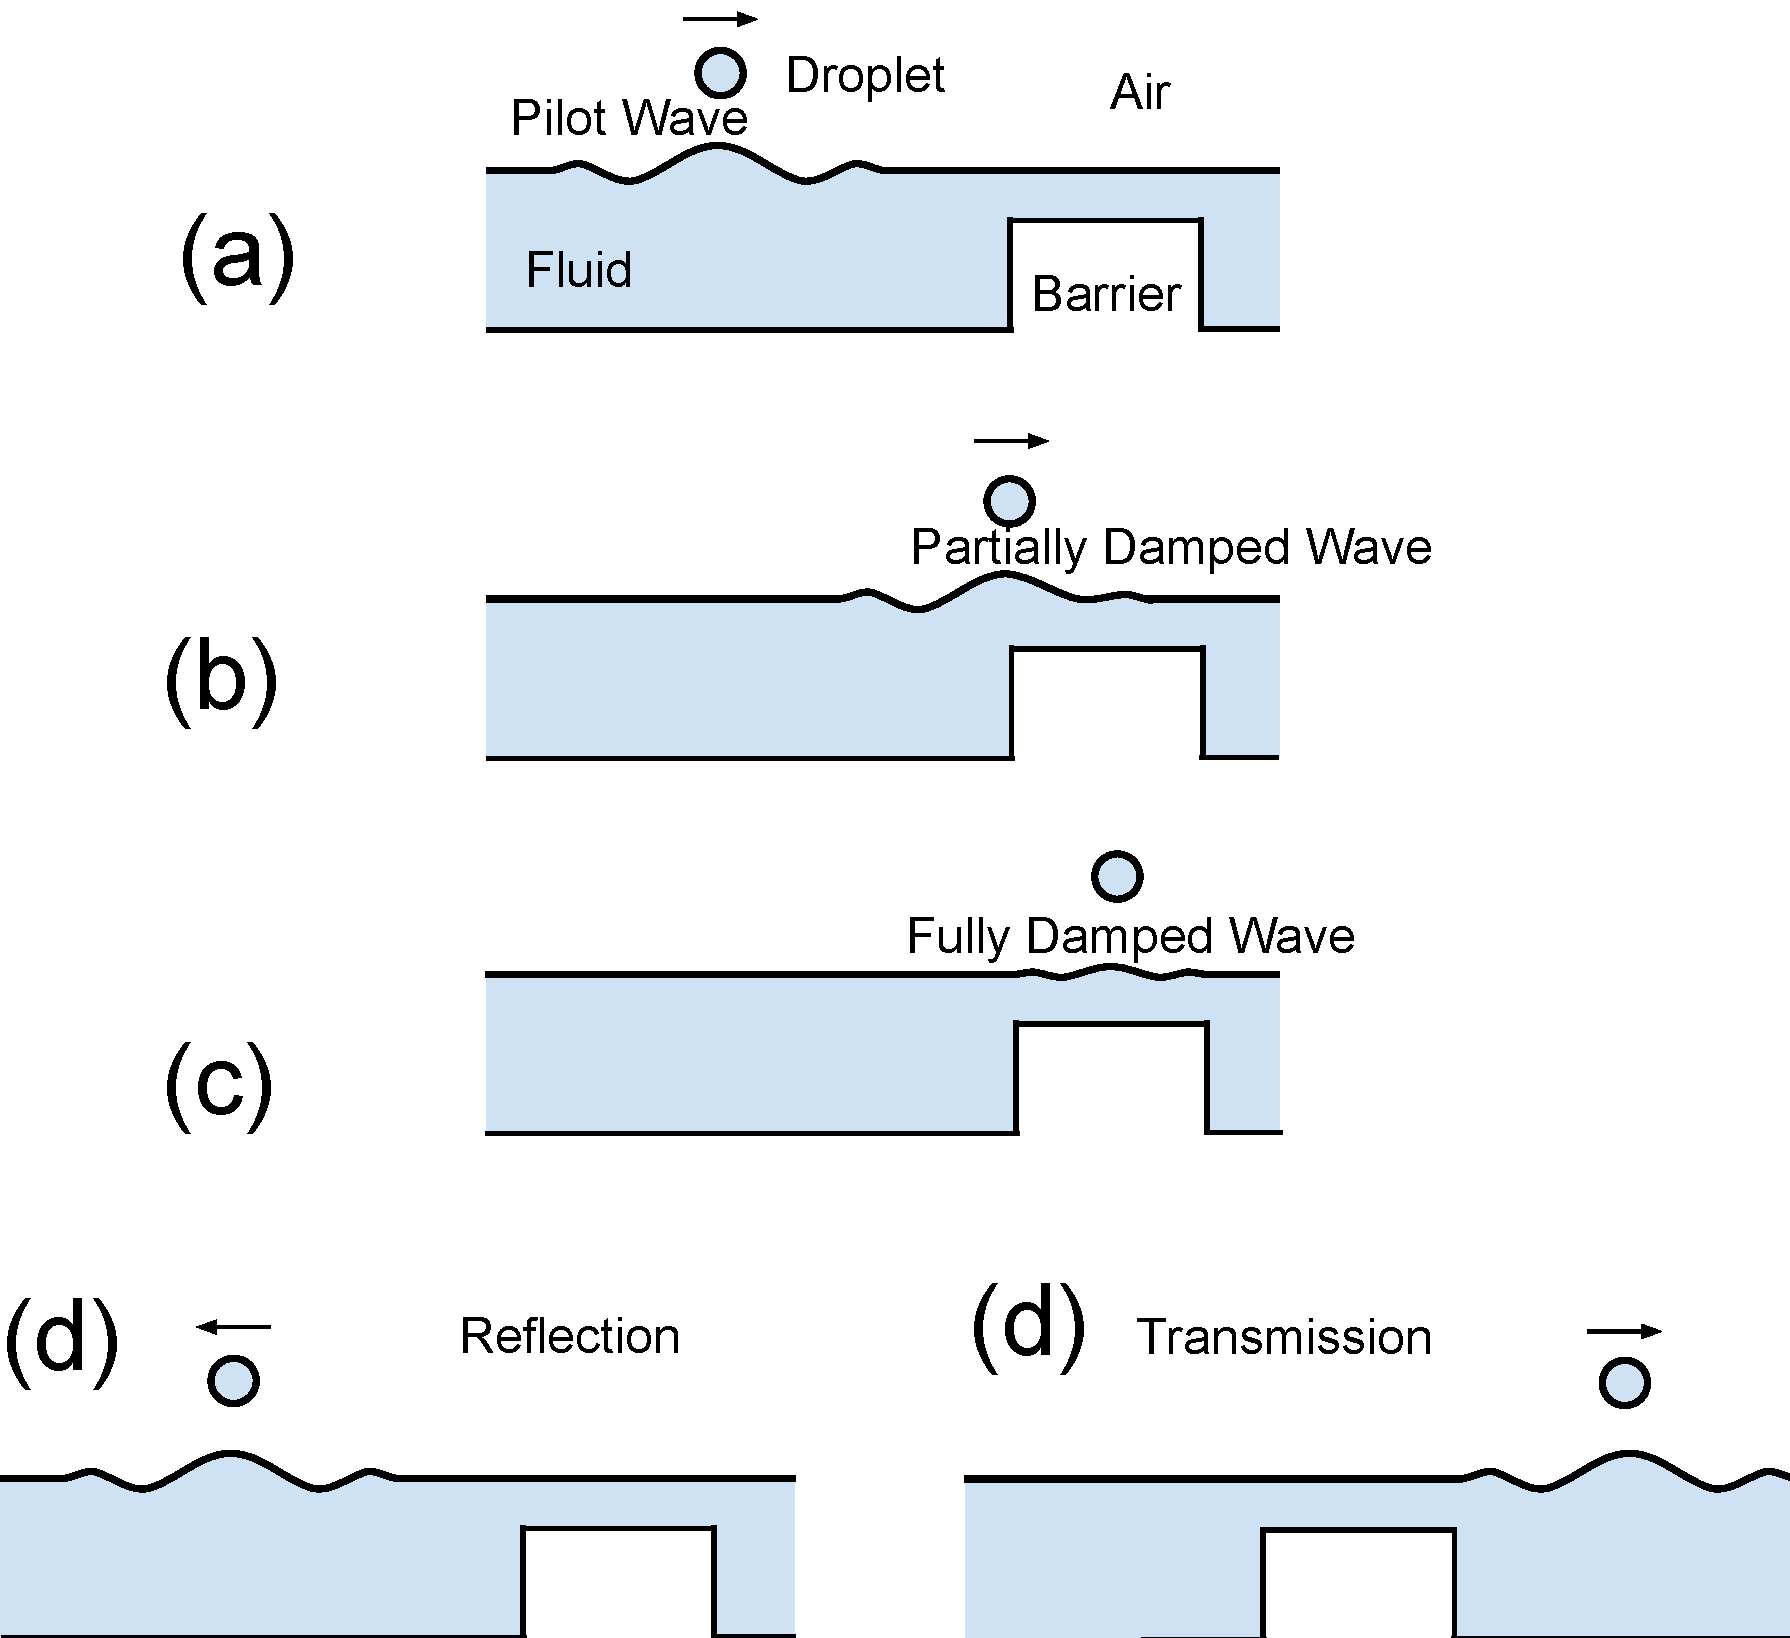
\includegraphics[scale=0.5]{Tunneling}
	     \caption{A diagram of the droplet-barrier interaction. In (a) the walker moves towards the barrier. As it gets closer (b), the guiding wave is damped. In (c) the guiding wave is fully damped such that the droplet is no longer a walker but a bouncer. Guided by the waves the droplet generated as a walker, the bouncer will either be reflected back from where it came (d), or carry on as shown in (e).}
	 \label{tuncartoon}
	\end{figure}
	A study performed by Eddi et al. examined tunneling in the bouncing droplet system \cite{tunneling}. In this setting, tunneling takes the form of the droplet tunneling through (or being reflected by) a subsurface barrier. The droplet never actually travels through the barrier, since it bounces on the interface, but the analog to quantum tunneling remains, because as the droplet approaches the barrier it is affected by the region of a different ``potential". 
	
For a different depth of fluid $H$, a tray will have a different $\gamma_\mathrm{W}$. If a tray has various regions of different depths, then these different regions will behave slightly differently. This means that when a walker travels from an area of one depth to an area of another depth, its behavior may change. This effect can be seen when a walker is pushed back from an under-the-surface step, seemingly without any contact with the droplet. However, in certain cases, the walker will actually ``tunnel" across the step; that is, it will continue to walk along the surface of the oil bath and pass into the new region of different depth, without reflection. Adjusting the width of the region as well as its depth will affect the behavior of the droplet. If we make this region of the tray of width $e$ with depth $h$ in a bath that otherwise has depth $H$, then we can think of if as a potential barrier. The unpredictability of the tunneling comes from the complex interaction between the drop and its guiding wave. 

Now say we set $\gamma$ such that walking occurs in the deeper section, but not in the more shallow section (i.e.  $\gamma_\mathrm{W}(H)<\gamma<\gamma_\mathrm{W}(h)$.) Then, the droplet is simply a bouncer when on the shallow region, but a walker everywhere else. If the droplet starts out in the deeper region but crosses over to the shallow barrier, its behavior becomes slow since it is no longer generating the self-propelling waves required for the walking motion. Instead, the superposition of previous waves is what guides it either through or away from the barrier. However, if a droplet were to be created on the barrier, it would remain motionless. We understand the act of tunneling to be: the walker approaches a barrier, crosses the barrier as a bouncer, and eventually returns to the deeper region as a walker. The process is depicted in \refFig{tuncartoon}. 

\begin{figure}[]
  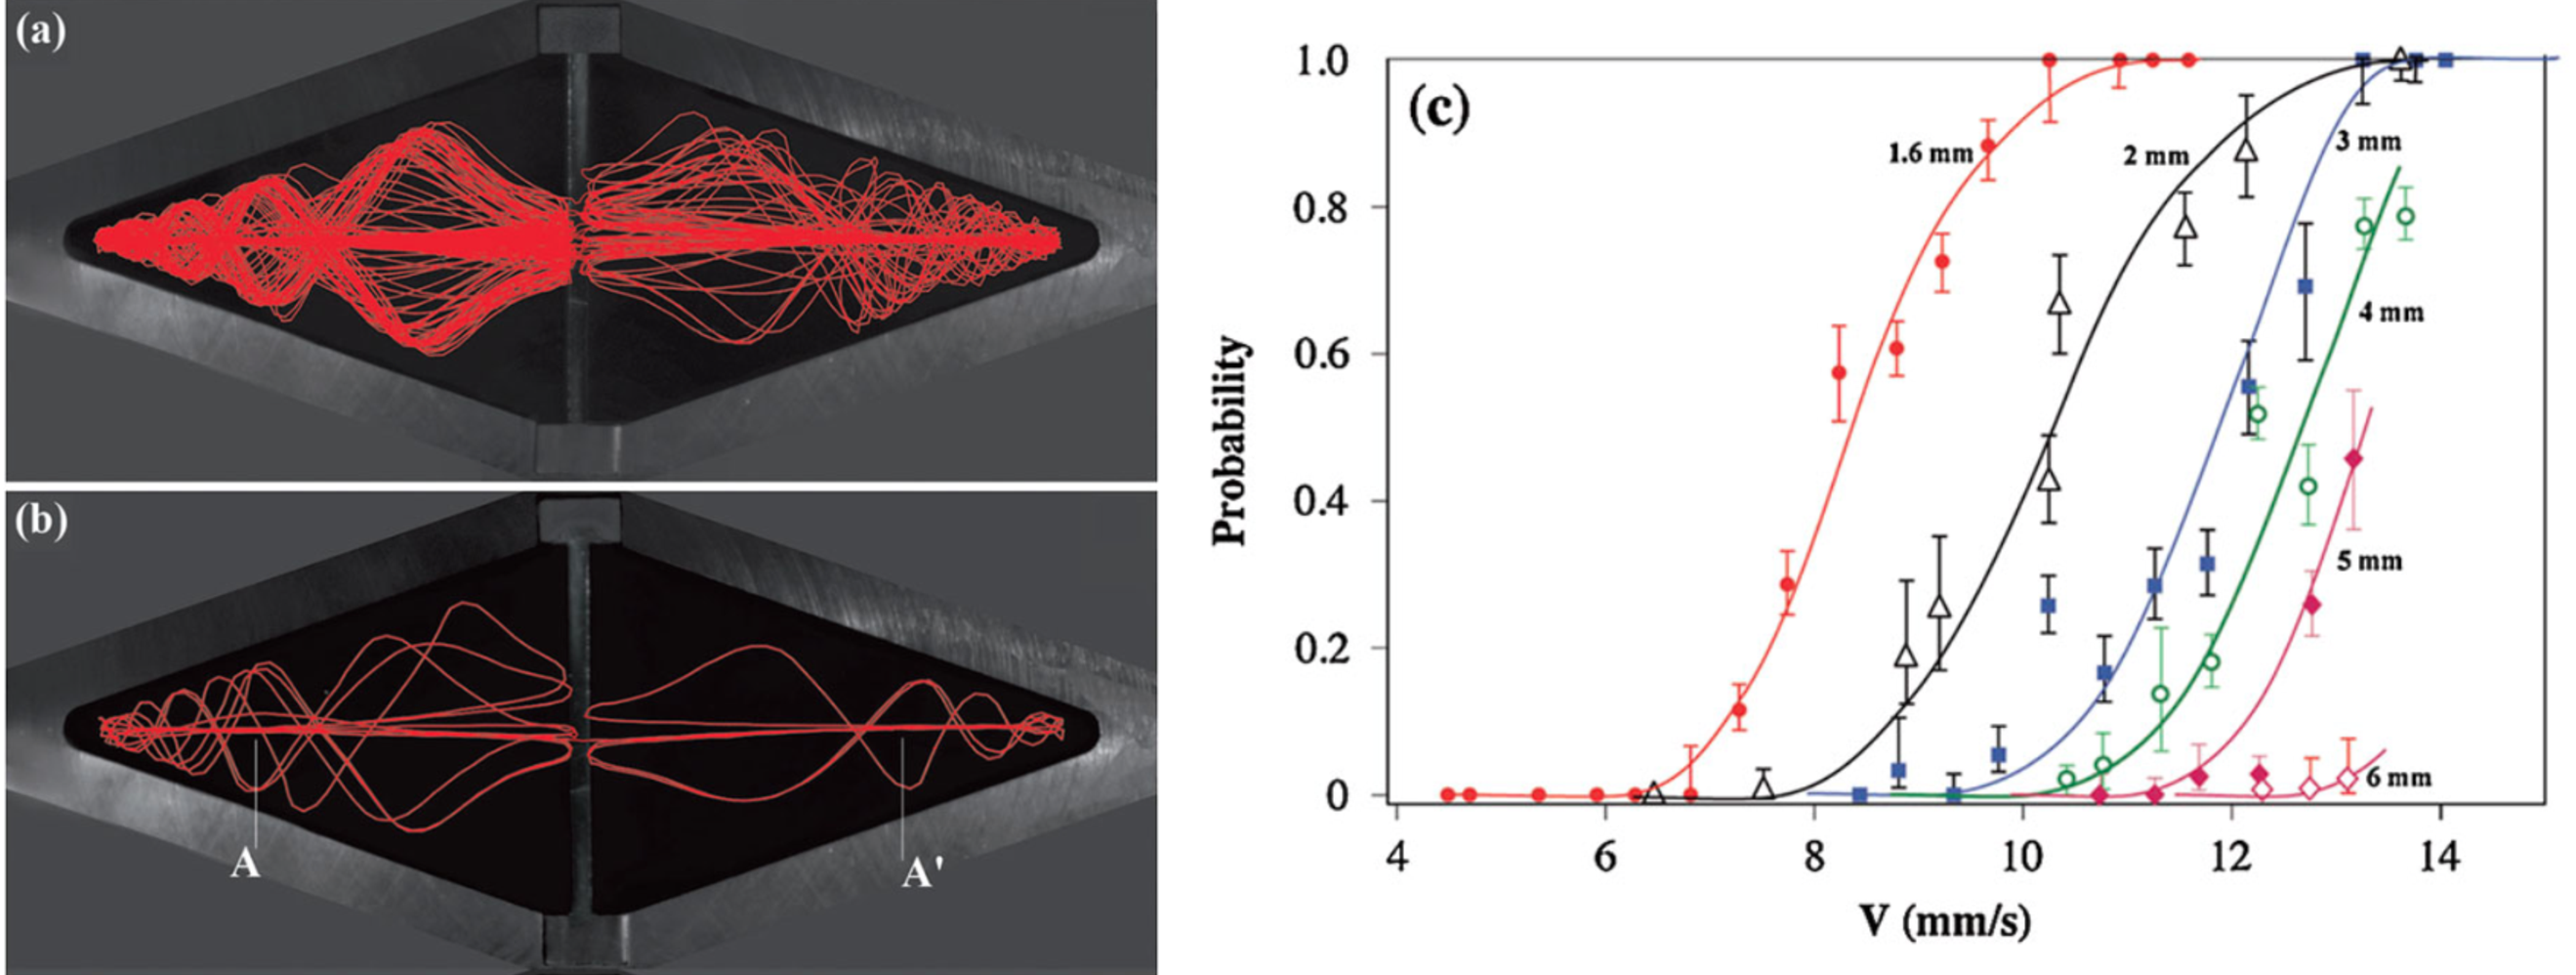
\includegraphics[width=1.0\linewidth]{EddiCombo}
\caption{In (a) and (b) we see the path of a droplet traced out over many collisions with the barrier in then rhombus shaped tray. The plot (c) shows the tunneling probability as a function of walker velocity for different barrier widths. Figures from A. Eddi, Phys. Rev. Lett. \textbf{102}, 240401-3 (2009).}
\label{fig:Eddi}
	\end{figure}

Eddi et al. built a tray with a submerged rhombus shape (of inner lengths $120~\mathrm{mm}$ by $45~\mathrm{mm}$) which forced the walker across the center of the tray shown in \refFig{fig:Eddi} (a) - (b). A barrier was then placed along the diagonal of the rhombus, perpendicular to the direction of travel of the walker, so that the walker would run directly into the wall. Their experiment was conducted in a bath depth $H = 4.1~\mathrm{mm}$, a barrier depth $h = 1.1~\mathrm{mm}$, and with barriers of width $e = 1.6, 2, 3, 4, 5 $ and $ 6~\mathrm{mm}$. They showed that as $\gamma/\gamma_\mathrm{F}$ approached $1$, faster droplets had higher probabilities of tunneling (\refFig{fig:Eddi} (c)). They also discovered that by increasing the barrier width, the tunneling probability decreased. 

The question that lingers, and that is the focus of this thesis, is the following: \textbf{how does tunneling probability change as a function of oil depth above the barrier $h$?} We expect that at large $h$ values, walkers will tunnel through very frequently, and at small values of $h$, there will be very little tunneling. What is the critical height where we see both behaviors? An experiment with a value of $h = 1.1~\mathrm{mm}$, as performed in the aforementioned study, would be a good starting place. 